
\documentclass[12pt]{article} % article class, 12pt font

% load any packages you need for more custom stuff
\usepackage[margin=1in]{geometry} % set 1-inch margins
\usepackage{setspace}\doublespacing % set double spacing
\usepackage[superscript]{cite} % superscript numeric in-line citations
\usepackage{indentfirst} % indent the first paragraph of each section
\usepackage{graphicx} % enable displaying png format graphs
\usepackage{csvsimple} % enable importing tabular data
\usepackage{booktabs} % enable formulating tables


% set title stuff
\title{The Spread of Disease}
\newcommand{\authors}{Eli Sylvia-Lourde}
\author{Math 114 Mathematical Modeling\\St. Mary's College}
\date{February 22, 2019}

% start the actual document
\begin{document}

% create title stuff
\hfill\authors % write the authors right-aligned
%\vspace{-0.5in} % reduce space before title
{\let\newpage\relax\maketitle} % print title

% begin the main text
\section*{Problem Statement}
An	isolated	town	has	a	population	of	100,000	residents.	Last	week	there	were	18 new	cases	of
people	infected	by	a	mild	disease	that	lasts three	weeks and	leaves	the	person	immune	from
further	disease.	Direct	contact	with	an	infected person	leads	to	an	infection	of	a	previously
uninfected	person.	This	week	there	are	40 new	cases.	It	is	estimated	that	30\% of	the	existing
population	is	immune	because	of	previous	exposure.

\begin{enumerate}
\item
Make	a	list	of	assumptions	that	you	need	to	make	in	order	to	develop	a	dynamical
system	model	using	difference	equations.
\item
Develop	a	model	that	describes	how	the	number	of	new	cases	each	week	develops.
\item
What	is	the	eventual number	of	people	who	will	become	infected?
\item
Vary	the	assumptions	you	make	in	this	model	to	develop	a	feel	for	how	sensitive	the
model	is	to	your	assumptions.
\end{enumerate}

\section*{List of Assumptions}
\begin{itemize}
\item
Every person in the population is equally exposed to any peoples that are infected.
\item
Every person that is exposed to an individual that is infected has the same chance of becoming infected themselves.
\item
 During the 0th week the infection is introduced into the population, 18
people develop cases of the sickness.
\item
During the first week the infection is introduced into the population, 40
people develop cases of the sickness.
\item
People recover on their third week on getting the disease, not after their third week of getting the disease.
\item
That the 30\% of people that are immune in week 2 represent the only people of the population that are immune.
\end{enumerate}

\section*{The Model}
Based upon an equation given by the book, (Section 1.2|Example 3|p.13) we can assume that the spread of
disease can be modeled with the following equation: \linebreak $\Delta i_{n} = i_{n+1} - i_{n} = ki_{n}(N-i_{n})$
, where $i_{n}$ is the number of people that developed the disease on week $n$, $k$ is a constant, and $N$ is the total
population. In this equation, $i_{n}(N-i_{n})$ represents the number of times an infected person will come into contact with someone who can become sick. $k$ is the probability that someone will become sick if they encounter someone that is infected. Unlike the equation in the book, the people in the problem statement will get better after 3 weeks of having the disease. Also, we don't only care about the spread of disease, but rather the total number of people that are infected. This is reflected in the following equation:
 $ \displaystyle i_{n+1} = i_{n} + ki_{n}(N-i_{n}-s_{n}) - \Delta i_{n-2}$.
This reads as the following: the number of people that have the disease in week n+1 is equal to the number of people that have the disease in week n plus the number of people that contracted the disease in week n+1, minus the number of people that have become immune to the disease. The number of people that have contracted the disease is calculated by multiplying the constant k, the number of people that had the disease on week n, and the number of people that are succeptible to the disease. The number of people succeptible to the disease is found by subtracting the number of sick people on week n and the number of immune people on week n. We can determine our constant k by calculating the number of people that become infected on week 1. We do so with the following formula, using the data that we were given in the problem statement:

\[40 = (100,000 - 100,000*0.3 - 18) \]
\[k = 3.1754197111003146E-5 \]

Each week, we calculate the number of people that developed the disease, the number of people that became immune to the disease, the total number of infected, the total number of those that are immune, and the total number of those that are susceptible.

We calculate the total number of people that developed a new case of the disease by using a formula that is similar to the one we used to solve for K:
\[\Delta I_{n} = S_{n}*I_{n}*k-\Delta P_{n}\]
Where $\Delta I_{n}$ represents the change in the infected population, $S_{n}$ represents the number of people that are susceptible at week $n$, $I_{n}$ represents the number of people that are infected for week $n$, $k$ is our constant, and $\Delta P_{n}$ represents the number of people that became immune and are now protected from the disease at week $n$, which is the same as $\Delta I_{n-3}$. We record how many people are immune at week $n$ by adding $\Delta I_{n-3}$ to  After we calculate how many people developed the disease, we then calculate how many people developed immunity. This can be done by calculating $\Delta I_{n-3}$. Using these two numbers, we calculate how many people have the disease on week $n$. Finally, we use the new data to calculate the number of people that are now susceptible to the disease, which is equivalent to: $S_{n} = S_{n-1} + \Delta I_{n} - \Delta I_{n-3} $ Using these data points, we are now able to watch the disease take its course through the population.

\section*{Findings}
When running the model, we get the following data:

% \csvautobooktabular[table head=\toprule\bfseries Week & \bfseries Infected \bfseries Delta Infected \\\midrule\csvlinetotablerow\\]{Disease_Data.csv}
% \csvautobooktabular[table head=\toprule\bfseries Week & \bfseries Infected \bfseries Delta Infected \\\midrule\csvlinetotablerow\\]{Disease_Data.csv}
{\centering
\csvautobooktabular{Disease_Data.csv}
\\}



% 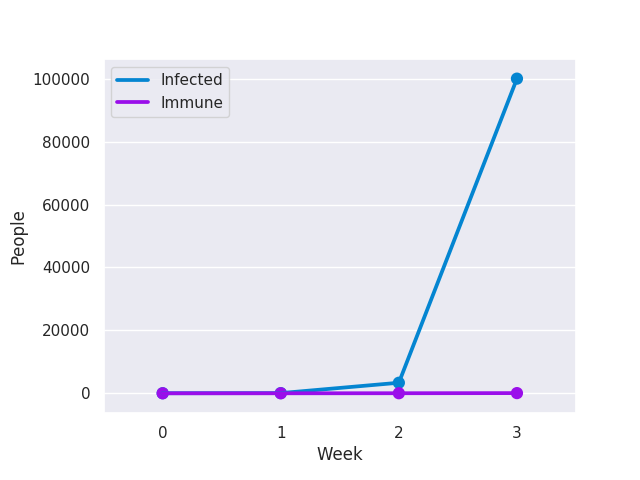
\includegraphics{Actual_Spread.png}
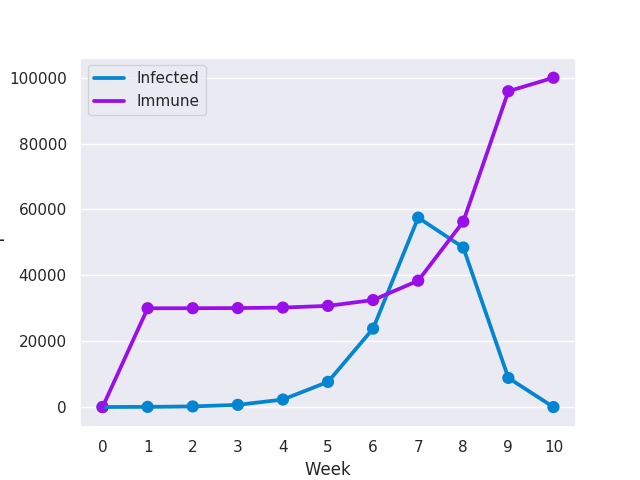
\includegraphics{Spread_Of_Disease.png}
The graph is built from the data table above. As we can see, the number of sick people peaks at 5,657.911, which we could round up to 5,657 or 5,658. The only way for the virus to not infect everyone is if we decrease k by a magnitude of 10, which results in the chart below:
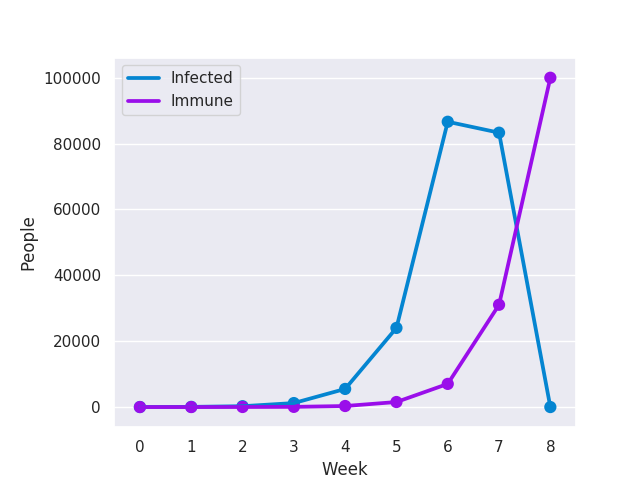
\includegraphics{humans_win.png}
It would be interesting to see what happens if we implement death into the model, where 5\% of those that are infected fall victim to the disease. It would also be interesting to change up the delta equation, that is to vary the probability of someone in the population developing the disease. This sort of thing could also be done with respect to how the infected interact with those that are immune. We could assign a range of ages to those in the population and give each each bracket another range of immune system ratings as well as a number of interactions with those that are infected.

\end{document} % this ends your document
